% Editable source for result.pdf, written by make_figures.py from the run's result.json
\documentclass[tikz,border=6pt]{standalone}
\usepackage[T1]{fontenc}
\begin{document}
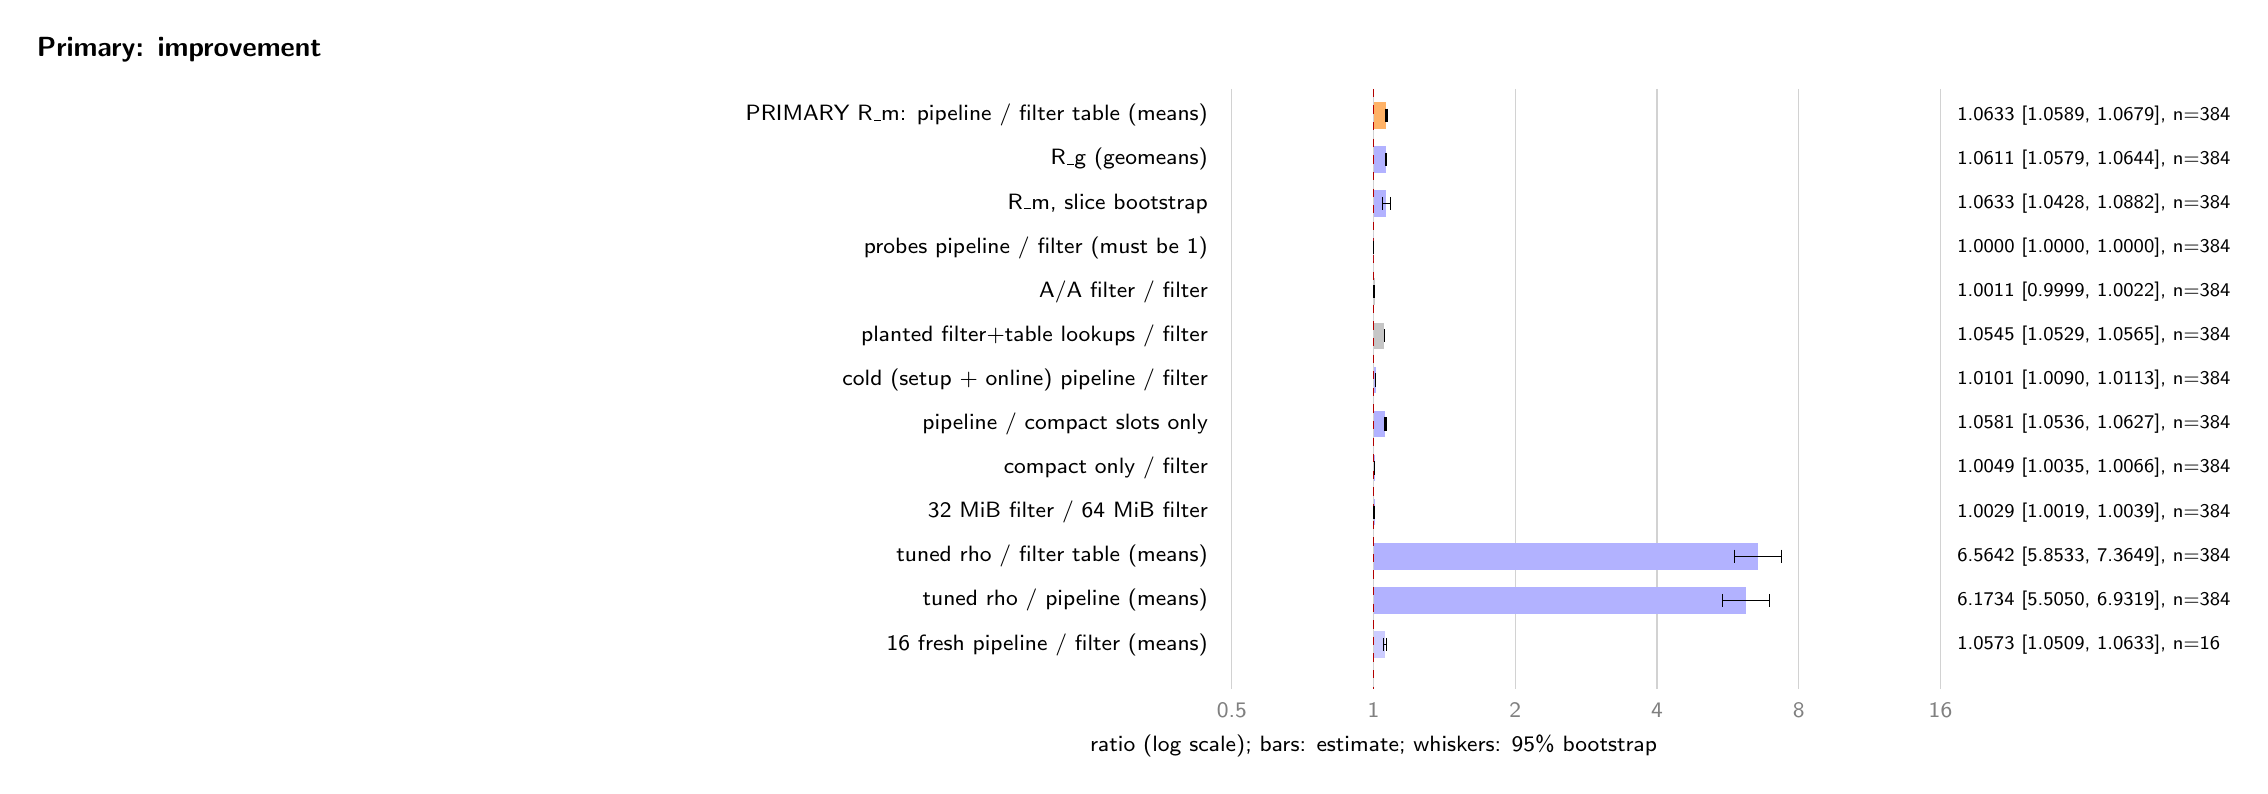
\begin{tikzpicture}[font=\sffamily\footnotesize,x=18mm,y=-5.6mm]
\draw[gray!35] (-1.0000,-0.6) -- (-1.0000,13); \node[gray] at (-1.0000,13.5) {0.5};
\draw[gray!35] (0.0000,-0.6) -- (0.0000,13); \node[gray] at (0.0000,13.5) {1};
\draw[gray!35] (1.0000,-0.6) -- (1.0000,13); \node[gray] at (1.0000,13.5) {2};
\draw[gray!35] (2.0000,-0.6) -- (2.0000,13); \node[gray] at (2.0000,13.5) {4};
\draw[gray!35] (3.0000,-0.6) -- (3.0000,13); \node[gray] at (3.0000,13.5) {8};
\draw[gray!35] (4.0000,-0.6) -- (4.0000,13); \node[gray] at (4.0000,13.5) {16};
\draw[red!70!black,dashed] (0,-0.6) -- (0,13);
\node at (0,14.3) {ratio (log scale); bars: estimate; whiskers: 95\% bootstrap};
\node[anchor=west,font=\sffamily\bfseries] at (-9.5,-1.5) {Primary: improvement};
\node[anchor=east] at (-1.1000,0) {PRIMARY R\_m: pipeline / filter table (means)};
\fill[orange!60] (0,-0.300000) rectangle (0.0885,0.300000);
\draw (0.0826,0) -- (0.0948,0); \draw (0.0826,-0.150000) -- (0.0826,0.150000); \draw (0.0948,-0.150000) -- (0.0948,0.150000);
\node[anchor=west,font=\sffamily\scriptsize] at (4.0500,0) {1.0633 [1.0589, 1.0679], n=384};
\node[anchor=east] at (-1.1000,1) {R\_g (geomeans)};
\fill[blue!30] (0,0.700000) rectangle (0.0856,1.300000);
\draw (0.0812,1) -- (0.0900,1); \draw (0.0812,0.850000) -- (0.0812,1.150000); \draw (0.0900,0.850000) -- (0.0900,1.150000);
\node[anchor=west,font=\sffamily\scriptsize] at (4.0500,1) {1.0611 [1.0579, 1.0644], n=384};
\node[anchor=east] at (-1.1000,2) {R\_m, slice bootstrap};
\fill[blue!30] (0,1.700000) rectangle (0.0885,2.300000);
\draw (0.0605,2) -- (0.1219,2); \draw (0.0605,1.850000) -- (0.0605,2.150000); \draw (0.1219,1.850000) -- (0.1219,2.150000);
\node[anchor=west,font=\sffamily\scriptsize] at (4.0500,2) {1.0633 [1.0428, 1.0882], n=384};
\node[anchor=east] at (-1.1000,3) {probes pipeline / filter (must be 1)};
\fill[blue!30] (0,2.700000) rectangle (0.0000,3.300000);
\draw (0.0000,3) -- (0.0000,3); \draw (0.0000,2.850000) -- (0.0000,3.150000); \draw (0.0000,2.850000) -- (0.0000,3.150000);
\node[anchor=west,font=\sffamily\scriptsize] at (4.0500,3) {1.0000 [1.0000, 1.0000], n=384};
\node[anchor=east] at (-1.1000,4) {A/A filter / filter};
\fill[gray!45] (0,3.700000) rectangle (0.0015,4.300000);
\draw (-0.0002,4) -- (0.0031,4); \draw (-0.0002,3.850000) -- (-0.0002,4.150000); \draw (0.0031,3.850000) -- (0.0031,4.150000);
\node[anchor=west,font=\sffamily\scriptsize] at (4.0500,4) {1.0011 [0.9999, 1.0022], n=384};
\node[anchor=east] at (-1.1000,5) {planted filter+table lookups / filter};
\fill[gray!45] (0,4.700000) rectangle (0.0766,5.300000);
\draw (0.0743,5) -- (0.0793,5); \draw (0.0743,4.850000) -- (0.0743,5.150000); \draw (0.0793,4.850000) -- (0.0793,5.150000);
\node[anchor=west,font=\sffamily\scriptsize] at (4.0500,5) {1.0545 [1.0529, 1.0565], n=384};
\node[anchor=east] at (-1.1000,6) {cold (setup + online) pipeline / filter};
\fill[blue!30] (0,5.700000) rectangle (0.0145,6.300000);
\draw (0.0129,6) -- (0.0162,6); \draw (0.0129,5.850000) -- (0.0129,6.150000); \draw (0.0162,5.850000) -- (0.0162,6.150000);
\node[anchor=west,font=\sffamily\scriptsize] at (4.0500,6) {1.0101 [1.0090, 1.0113], n=384};
\node[anchor=east] at (-1.1000,7) {pipeline / compact slots only};
\fill[blue!30] (0,6.700000) rectangle (0.0815,7.300000);
\draw (0.0753,7) -- (0.0878,7); \draw (0.0753,6.850000) -- (0.0753,7.150000); \draw (0.0878,6.850000) -- (0.0878,7.150000);
\node[anchor=west,font=\sffamily\scriptsize] at (4.0500,7) {1.0581 [1.0536, 1.0627], n=384};
\node[anchor=east] at (-1.1000,8) {compact only / filter};
\fill[blue!30] (0,7.700000) rectangle (0.0070,8.300000);
\draw (0.0050,8) -- (0.0096,8); \draw (0.0050,7.850000) -- (0.0050,8.150000); \draw (0.0096,7.850000) -- (0.0096,8.150000);
\node[anchor=west,font=\sffamily\scriptsize] at (4.0500,8) {1.0049 [1.0035, 1.0066], n=384};
\node[anchor=east] at (-1.1000,9) {32 MiB filter / 64 MiB filter};
\fill[blue!30] (0,8.700000) rectangle (0.0042,9.300000);
\draw (0.0027,9) -- (0.0056,9); \draw (0.0027,8.850000) -- (0.0027,9.150000); \draw (0.0056,8.850000) -- (0.0056,9.150000);
\node[anchor=west,font=\sffamily\scriptsize] at (4.0500,9) {1.0029 [1.0019, 1.0039], n=384};
\node[anchor=east] at (-1.1000,10) {tuned rho / filter table (means)};
\fill[blue!30] (0,9.700000) rectangle (2.7146,10.300000);
\draw (2.5492,10) -- (2.8807,10); \draw (2.5492,9.850000) -- (2.5492,10.150000); \draw (2.8807,9.850000) -- (2.8807,10.150000);
\node[anchor=west,font=\sffamily\scriptsize] at (4.0500,10) {6.5642 [5.8533, 7.3649], n=384};
\node[anchor=east] at (-1.1000,11) {tuned rho / pipeline (means)};
\fill[blue!30] (0,10.700000) rectangle (2.6261,11.300000);
\draw (2.4607,11) -- (2.7933,11); \draw (2.4607,10.850000) -- (2.4607,11.150000); \draw (2.7933,10.850000) -- (2.7933,11.150000);
\node[anchor=west,font=\sffamily\scriptsize] at (4.0500,11) {6.1734 [5.5050, 6.9319], n=384};
\node[anchor=east] at (-1.1000,12) {16 fresh pipeline / filter (means)};
\fill[blue!20] (0,11.700000) rectangle (0.0804,12.300000);
\draw (0.0717,12) -- (0.0886,12); \draw (0.0717,11.850000) -- (0.0717,12.150000); \draw (0.0886,11.850000) -- (0.0886,12.150000);
\node[anchor=west,font=\sffamily\scriptsize] at (4.0500,12) {1.0573 [1.0509, 1.0633], n=16};
\end{tikzpicture}
\end{document}
